\documentclass[10pt, french]{article} 
\usepackage[utf8]{inputenc}

% 10pt permet de déterminer la taille de la fonte
\usepackage[utf8]{inputenc}

\usepackage{amssymb,amsmath,amsthm,amsfonts, bbm} 
% il s'agit de différents packages utilisés pour écrire des mathématiques en Latex

\usepackage{geometry}
\geometry{hmargin=2.3cm,vmargin=2.5cm}
% ce package permet de spécifier la taille des marges (h: horizontales; v: verticales)
\usepackage{babel}
\usepackage{array}
\usepackage{graphicx,graphics}
\usepackage{caption}
\usepackage{subcaption}
\usepackage[svgnames]{xcolor}
\usepackage{stmaryrd}
\usepackage{dsfont}
\usepackage{titling}
\usepackage{pdfpages}
\usepackage{amsmath}
\usepackage{amsfonts}
\usepackage{epsfig}
\usepackage{listings}

\usepackage[section]{placeins}
% packages utilisés pour faire des tableaux, graphiques et mise en page

\usepackage{url}
\lstset{language = Python,
inputencoding=utf8,
    extendedchars=true,
    literate={á}{{\'a}}1 {ã}{{\~a}}1 {é}{{\'e}}1 {è}{{\`e}}1 {à}{{\`a}}1 {ô}{{\^o}}1 {ù}{{\`u}}1,
    backgroundcolor=\color{WhiteSmoke},   
    commentstyle=\color{DarkOrange},
    keywordstyle=\color{NavyBlue},
    numberstyle=\tiny\color{LightSlateGrey},
    stringstyle=\color{MediumVioletRed},
    basicstyle=\footnotesize\color{DarkSlateGrey},
    breakatwhitespace=false,         
    breaklines=true,                 
    captionpos=b,                    
    keepspaces=true,                 
    numbers=left,                    
    numbersep=5pt,                  
    showspaces=false,                
    showstringspaces=false,
    showtabs=false,                  
    tabsize=2,}



\title{Compte-rendu Projet Python: \\ Création d'une intelligence artificielle pour le Tic Tac Toe $9\times9$ }
\author{Pierre Eustache - Laure-Hélène Genuyt }
\date{21 mai 2018}

\begin{document}

\maketitle
\tableofcontents
%\section{Objectifs du rapport}
 %Le rapport doit contenir les éléments suivants :

%\begin{itemize}
 %   \item instructions pour exécuter le programme

%\item description d’un point de design de code
%\item
%description d’un algorithme du programme et son coût
%\item
%description d’une difficulté qui vous a fait perdre beaucoup de temps (hors celles liées à votre apprentissage de la programmation)
%\item
%description d’une contribution originale
%\item
%description des résultats obtenus
%\item
%prolongements et applications envisageables

%\end{itemize}
\paragraph{}
    
\section{Introduction}
\par L'objectif de ce projet a été de créer une intelligence artificielle pour le jeu du Tic Tac Toe $9\times9$ (aussi appelé morpionception, ou Ultimate Tic Tac Toe). \\
\par Ce projet nous a permis de mieux comprendre le monde des intelligences artificielles, en en explorant différentes formes (algorithme génétique, algorithme minimax...). 
Il nous également permis d'apprendre à réaliser une interface graphique, en utilisant le package \textit{tkinter} de python. \\
\par Enfin, le fait de réussir à produire une version numérique du jeu, avec une interface graphique permettant à un joueur humain de jouer contre une intelligence artificielle, nous a donné la satisfaction d'avoir réellement "créé" quelque chose grâce à la programmation. 
\paragraph{}



    
\subsection*{Le jeu}
\begin{enumerate}
    \item \textbf{Règles du jeu} 


\par Il s'agit d'un jeu de plateau, composé d'une grille de 3 cases par 3, dont chacune des cases contient elle-même une grille de 3 par 3. Dans la suite, on se référera à la "grande grille" et aux "petites grilles" pour distinguer ces deux niveaux de jeu.\\
\par L'objectif du jeu est de remporter 3 cases de la grande grille, en y apposant son symbole (une croix ou un cercle). Pour cela, les joueurs jouent au niveau des petites grilles, et cherchent à les remporter en alignant 3 de leurs symboles. Une fois la petite grille gagnée, on ne peut plus y jouer, et elle devient elle-même une case "croix" ou "cercle". \\
\par Le jeu présente cependant une subtilité qui le rend intéressant: chaque joueur doit jouer dans la case de la grande grille correspondant à la case de la petite grille où a joué l'autre joueur au tour précédent.


%\paragraph{}
%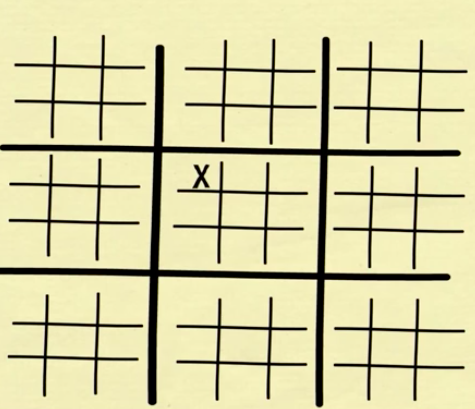
\includegraphics[width=0.25\textwidth]{tour1.png}
%\caption{Joueur A a joué dans la case en haut à gauche d'une petite grille} \\
%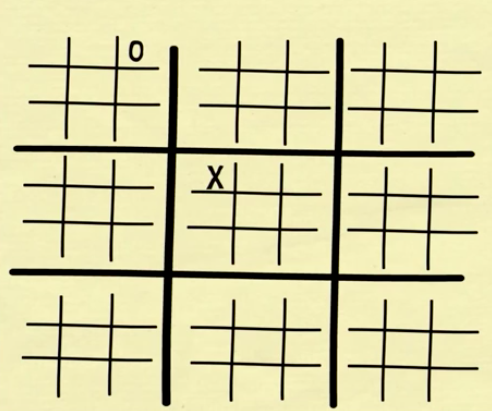
\includegraphics[width=0.25\textwidth]{tour2.png}
%\caption{Joueuer B doit donc jouer dans la case en haut à gauche de la grande grille} \\
%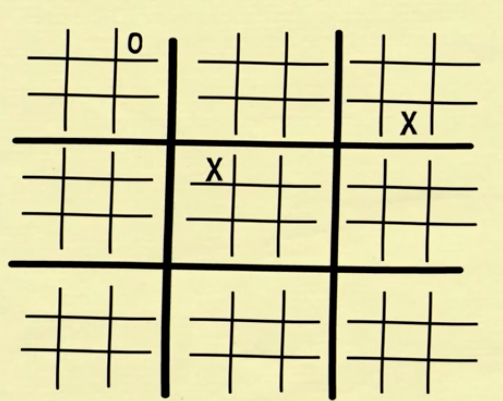
\includegraphics[width=0.25\textwidth]{tour3.png}
%\caption{Comme B a joué dans la case en haut à droite de sa petite grille, A doit jouer dans la case correspondante de la grande grille} \\
%\end{figure}


\begin{figure}
 \begin{minipage}[t]{0.25\linewidth}
  \centering\epsfig{figure = tour1.png,width=\linewidth}
  \caption{Dans cet exemple, A a joué dans la case en haut à gauche de sa petite grille.}
 \end{minipage} \hfill
 \begin{minipage}[t]{0.25\linewidth}
  \centering\epsfig{figure = tour2.png,width=\linewidth}
  \caption{Au tour suivant, B doit donc jouer dans la case en haut à gauche de la grande grille}
  \end{minipage} \hfill
 \begin{minipage}[t]{0.25\linewidth}
  \centering\epsfig{figure = tour3.png,width=\linewidth}
  \caption{Comme B a joué dans la case en haut à droite de sa petite grille, A doit ensuite jouer dans la case correspondante de la grande grille (etc.)}
 \end{minipage}
\end{figure}


\paragraph{}
Lorsqu'un joueur renvoie l'autre dans une case de la grande grille déjà gagnée, celui-ci peut jouer où il le souhaite. \\

Le jeu se termine dès qu'un joueur a réussi à aligner 3 croix ou 3 cercles dans des cases de la grande grille. 


\paragraph{}
\begin{figure}[h!]
\centering
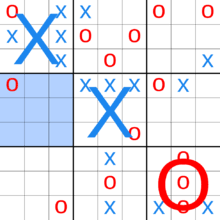
\includegraphics[width=0.5\textwidth]{exemple.png}
\caption{Exemple d'une partie de Tic Tac Toe $9\times9$}
\end{figure}

\item \textbf{Difficultés du jeu}

\par La création d'une intelligence artificielle pour ce jeu, en apparence relativement simple, pose quelques problèmes. 
En effet, contrairement au jeu du Tic Tac Toe classique, qui se termine par un match nul à moins d'une erreur d'inattention de la part d'un des joueurs, il est difficile de trouver une stratégie gagnante à ce jeu, et de bien en saisir tous les mécanismes.
\paragraph{}
De plus, la création d'une intelligence artificielle suppose de pouvoir évaluer chaque coup et de déterminer la valeur d'une position. Or, cela ne va pas de soi dans ce jeu, qui se joue à plusieurs niveaux: un coup doit-il être évalué à l'aune de ce qu'il apporte au joueur dans la petite grille où il est joué? \\
Ou faut-il davantage tenir compte de la case de la grande grille où il renvoie l'adversaire? 


\end{enumerate}

\paragraph{}
\section{Le projet}
\begin{figure}
\centering
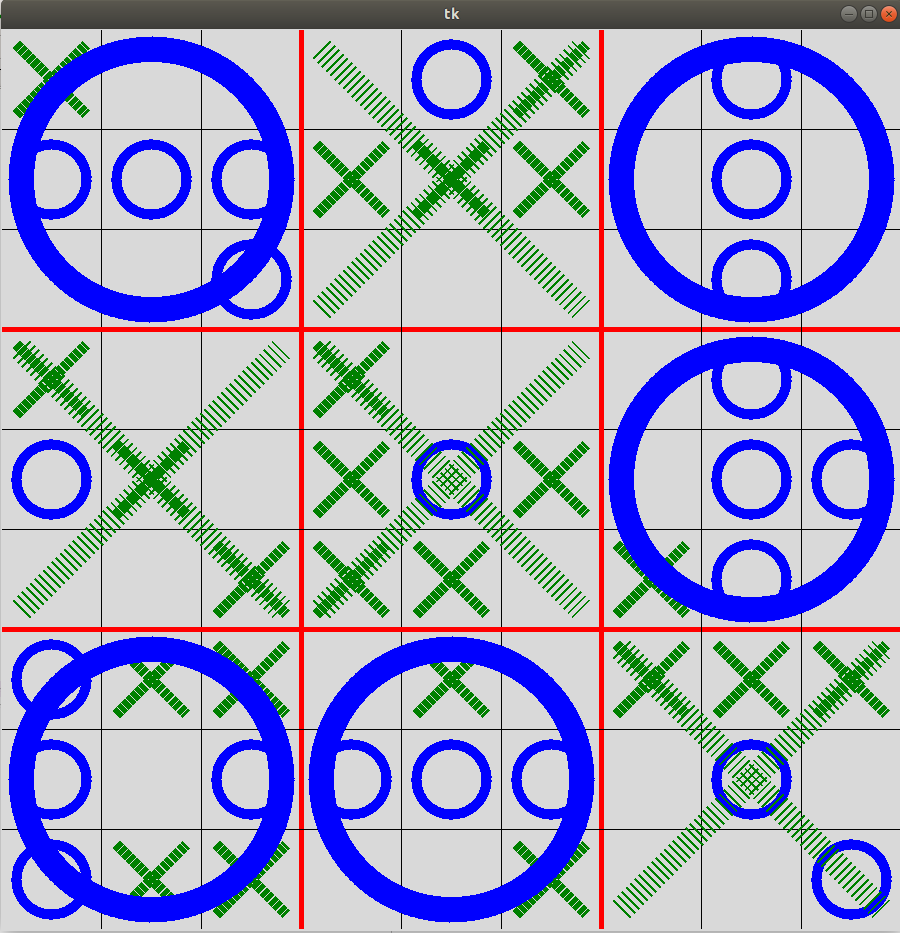
\includegraphics[width=.5\textwidth]{interface}
\caption{Le programme en action}
\end{figure}
\subsection{Le plan de route}

\begin{itemize}
    \item Nous avons tout d'abord réfléchi à une manière optimale de coder une partie, et plus particulièrement l'état de la grille à un instant donné. Nous avons décidé de répresenter  la grande grille comme un tableau $3\times3$ de tableaux $3\times3$ (les petites grilles). Chacune des 81 cases est donc référencée grâce à un quadruple indice. \\
    \par \underline{Ex}: la position (1,1,3,3) fait référence à la petite case en bas à droite de la grande case en haut à gauche. \\ 
    Notre tableau est composé de 0, de 1 et de 2, où 0 représente une case vide, 1 une case contenant une croix, et 2 une case contenant un cercle. \\
    \par Nous avons ensuite créé un algorithme permettant de coder ce tableau en binaire, afin d'optimiser l'espace pris par une grille, mais cela ne nous a finalement pas servi par la suite.
   \paragraph{}
    \item Nous nous sommes ensuite servis du module \textit{tkinter} pour créer une interface graphique affichant l'état de la grille à un instant donné, à partir du tableau décrit précédemment. 
    \paragraph{}
    \item Afin de créer notre intelligence artificielle, nous avons essayé d'évaluer la valeur d'un coup grâce à une analyse heuristique. 
    En effet, contrairement à un jeu d'échecs, où la valeur d'un coup peut être assimilé à la valeur du pion qu'il permet de prendre, il est difficile de trouver une valeur objective d'un coup au Tic Tac Toe $9\times9$. \\
    \par Nous avons donc créé une fonction prenant en compte un certain nombre d'indicateurs qui nous semblaient entrer dans l'évaluation d'un coup, et attribuant à chacun une pondération - déterminée d'après notre avis subjectif et notre expérience du jeu dans un premier temps. \\
    Ces indicateurs sont: 
    \begin{itemize}
        \item la case que l'on compte jouer se trouve-t-elle dans un coin? 
        \item se trouve-t-elle au centre d'une case? 
        \item se trouve-t-elle au bord d'une case? 
        \item combien de symboles a-t-on dans la grille où on renvoie l'adversaire?
        \item combien l'adversaire possède-t-il de symboles dans la grille où on le renvoie?  
        \item la case où on renvoie l'adversaire est-elle déjà gagnée?  
        \item cette case est-elle vide? 
        \item ce coup renvoie-t-il l'adversaire dans une case qu'il peut gagner? 
        \item ce coup permet-il de remporter la case? 
        \item ce coup permet-il de gagner le jeu? 
    \end{itemize}
\paragraph{}
Ces indicateurs ont une pondération positive si on juge qu'ils sont en faveur du joueur, négative si on juge le contraire. \\
On part par exemple du principe qu'il est plus avantageux de jouer au centre que dans un coin, et plus avantageux de jouer dans un coin que de jouer au bord. \\
On considère également qu'il vaut mieux renvoyer l'adversaire dans une case où il possède peu de symboles, et qu'il faut surtout éviter de l'envoyer dans une case déjà gagnée (ce qui lui permettrait de jouer n'importe où par la suite). 
\paragraph{}
\item Une fois cette heuristique créée, nous avons codé les règles du jeu (définition des coups possibles, enchaînement des actions, etc.), avant de créer une intelligence artificielle jouant aléatoirement selon ces règles (IA de type \textit{dummy} dans le code). 
\paragraph{}
\item Nous avons ensuite implémenté un algorithme génétique dans le but d'améliorer nos pondérations, et de créer une intelligence artificielle jouant selon ces pondérations. \\
\par La performance de ces intelligences artificielles (de type \textit{heurist} dans le code) a été évaluée en fonction de leur taux de victoire et de défaite contre l'intelligence artificielle jouant aléatoirement. 
L'algorithme génétique se décompose en plusieurs étapes: 
\begin{itemize}
    \item créer un lot de joueurs, jouant selon des pondérations déterminées de façon subjective dans un premier temps. 
    \item faire jouer ces joueurs contre notre intelligence artificielle aléatoire, en enregistrant leurs scores. 
    \item une fois le tournoi terminé, trier les joueurs selon leur score, et en garder la meilleure moitié. 
    \item muter le reste des joueurs, en modifiant de manière aléatoire leurs pondérations. 
    \item avec ce nouveau lot de joueurs (meilleure moitié et joueurs mutés), recommencer à partir de la deuxième étape.   
\end{itemize}

\item Au bout de 30 générations, nous avons obtenu les résultats suivants sur 100 matchs: 

On voit donc que notre intelligence artificielle générée par cet algorithme génétique présente une très nette amélioration par rapport à notre intelligence artificielle aléatoire.
$$
\begin{tabular}{ |c|c|c| }
\hline
Type & Heuristique & Aléatoire\\
\hline
Victoires & 91 & 35 \\
\hline
Nuls & 5 & 30 \\
\hline
 Défaites  & 4 & 35 \\
 \hline
\end{tabular}
$$
\\ 

\paragraph{}
\item Cette intelligence artificielle heuristique présente cependant une faiblesse majeure, qui est qu'elle n'a aucune profondeur dans son évaluation des coups: elle joue simplement selon des pondérations permettant d'évaluer la valeur du coup qu'elle va jouer \\
Nous avons donc implémenté un algorithme minimax, permettant à l'IA de voir à une profondeur de 3 coups. \\
\par Cet algorithme, que l'on peut représenter sous forme d'un arbre, examine toutes les évolutions possibles du jeu à partir de la configuration actuelle,et attribue à chacune de ces feuilles une valeur (selon les pondérations de la meilleure intelligence artificielle générée par l'algorithme génétique). \\
\par On considère que l'adversaire (qui joue au coup d'après), va choisir le coup qui l'amène à la situation la plus bénéfique pour lui, et donc la plus néfaste pour nous. \\
\par La valeur d'un noeud de l'adversaire correspond donc au minimum des feuilles évaluées précédemment. La valeur de chacun de nos coups possibles va donc être le maximum des valeurs des noeuds de l'adversaire, et on va jouer le coup possédant la plus haute valeur (il s'agit donc du coup qui nous permettra d'atteindre la situation de jeu la plus optimale pour nous dans 3 coups, en sachant que l'adversaire choisira toujours le coup qui lui est le plus avantageux).

\paragraph{}
\begin{figure}[h!]
\centering
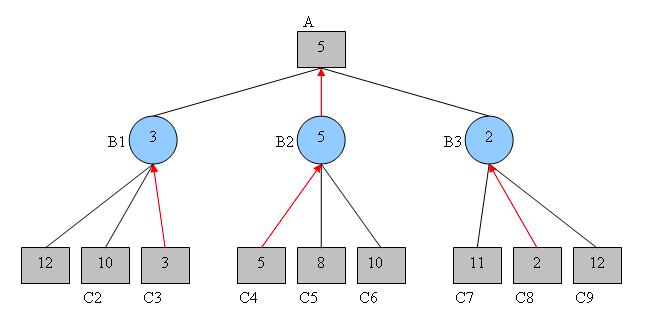
\includegraphics[width=0.7\textwidth]{minimax.png}
\caption{ }{Exemple d'arbre minimax (les carrés représentent ici les noeuds joueurs et les ronds les noeuds opposants)}
\end{figure}


Cet algorithme permet à l'intelligence artificielle (définie dans le code comme étant de type \textit{mini}) de gagner en performance. \\
Contre l'intelligence artificielle aléatoire, on a en effet observé, sur 200 matchs: 
$$
\begin{tabular}{ |c|c|c|c| }
\hline
Type & Minimax & Heuristique & Aléatoire\\
\hline
Victoires & 187 & 181 & 70 \\
\hline
Nuls & 10 & 10 & 60 \\
\hline
 Défaites & 3 & 8 & 70 \\
 \hline
\end{tabular}
$$

\paragraph{}
\item Une fois ces étapes réalisées, nous avons complété les classes \textit{Player} et\textit{Game}, permettant à chacune de définir les fonctions et les propriétés d'un joueur et d'une partie. 

\item In fine, notre programme permet donc: 
\begin{itemize}
    \item faire jouer deux intelligences artificielles (de type \textit{dummy}, \textit{eurist} ou \textit{mini}) l'une contre l'autre
    \item de jouer soi-même contre une intelligence artificielle de l'un de ces 3 types, sur une interface graphique adaptée.

\end{itemize}
\paragraph{}
$\Longrightarrow$ On a donc bien réussi à créer une intelligence artificielle pour le jeu du Tic Tac Toe $9\times9$, contre laquelle on peut jouer dans une interface graphique satisfaisante. \\
Si notre intelligence artificielle la plus satisfaisante (celle jouant selon l'algorithme minimax) est extrêmement performante contre une intelligence artificielle aléatoire, et constitue donc un réel succès sur ce point, elle s'avère cependant un peu faible face à un humain. \\
\par Cela est probablement dû à la difficulté d'évaluer simplement une situation de la grille à un moment donné, ainsi qu'à la difficulté qu'il y a à trouver une stratégie gagnante à ce jeu somme toute beaucoup moins simple qu'il n'y paraît. 



\end{itemize}

\subsection{Un point de design : la structure de données}
Le programme s'articule essentiellement autour de l'utilisation de deux classes : \emph{Player()} et 
\emph{Game()}.
\\
\begin{minipage}[]{.45\textwidth}
\begin{lstlisting}
class Game:
    def __init__(self,p1,p2):
        self.p1=p1 #ref the two players
        self.p2=p2
        self.mgrid=np.zeros((3,3),dtype=int) 
        self.grid=np.zeros((3,3,3,3),dtype=int)
        self.winner=0 
        self.actual=1 #actual player
        self.last=[3,3] #3,3 = no constrains
        self.dispo=np.ones((3,3,3,3), dtype=int)
        self.hist=[]   #keep an history
#        self.gagnable=np.ones((2,3,3),dtype=int)
        self.p1.tmpId=1 #sets for the player their order of turn
        self.p2.tmpId=2
        self.p1.gAct=self.p2.gAct=self #creates a ref to the game for the player
        self.turn=-1 #turn count
        self.mHist=np.zeros((3,3),dtype=int)-1 #hist for mGrid
        if self.p1.IA*self.p2.IA: self.auto_play() # plays
        elif self.p1.IA:
            self.versus(self.p2, self.p1)
        else: self.versus(self.p1, self.p2)
\end{lstlisting}
\end{minipage}
\begin{minipage}[]{.45\textwidth}
\begin{lstlisting}
class Player:
    name=0 #name by order of creation
    def __init__(self,pond=[3,2,1,1,1,1,1,1,1,1,1, math.inf],typ="heuri",IA=1):
        self.score=0 
        self.IA=IA
        self.name=Player.name
        Player.name+=1
        self.wins=0
        self.pond=np.array(pond) #heurisitic
        self.tmpId=0
        self.gAct=None
        self.typ=typ
        self.survival=0
       
    def move(self): #generic move function
        if self.typ=="dummy":
            return self.move1(self.gAct.grid, self.gAct.last, self.gAct.mgrid)
        if self.typ=="heuri":
            return self.move2()
        return self.move3(4)
\end{lstlisting}
\end{minipage}
\par Les méthodes sont pour beaucoup passées sous silence ici.
\par La partie est une instance de Game qui a pour attribut les deux joueurs. C'est également elle qui détient l'état du jeu au sens large, et l'historique des coups. Elle attribue à sa création une ID temporaire qui sert à distinguer les deux instances de joueurs de manière simple dans l'instance de chaque joueur. Elle enclenche ensuite une des deux méthodes de jeu en fonction du fait que les instances passées en argument soient ou non des joueurs
\paragraph{}



\paragraph{}
\subsection{L'algorithme génétique}
\subsubsection*{Description}
\begin{itemize}
    \item L'algorithme génétique consiste à répéter plusieurs fois les opérations suivantes: 
    \begin{itemize}
        \item créer une génération de joueurs
        \item les faire jouer plusieurs fois contre l'intelligence artificielle aléatoire  
        \item garder la meilleure moitié
        \item "muter" l'autre moitié, en modifiant aléatoirement les pondérations auxquelles ces joueurs obéissent 
        \item recommencer avec cette nouvelle génération
    \end{itemize}
    \paragraph{}
    Une étape de cet algorithme (soit une \textit{génération}, correspond à la fonction suivante: 
    \lstinputlisting[language = Python, firstline = 41, lastline = 47]{genetique.py}
    \paragraph{}
Cette fonction \textit{génération} fait elle-même appel à plusieurs autres fonctions, que nous allons détailler maintenant. 

\paragraph{}
\item La fonction \textit{génération} prend plusieurs arguments: 
\begin{itemize}
    \item n, qui correspond à la taille de l'échantillon de joueurs que nous allons considérer, et qui est ici fixé à 30
    \item nb, qui correspond au nombre de matchs que chacun de ces joueurs va faire contre l'intelligence artificielle aléatoire, et qui est ici fixé à 100
    \item N, qui correspond à la liste des joueurs 
\end{itemize}

\paragraph{}
\item À la première génération, N est encore vide. On crée donc un lot de joueurs, en faisant appel à la fonction \textit{create batch}: 
\lstinputlisting[language = Python, firstline = 10, lastline = 14]{genetique.py}
Cette fonction prend en argument n, la taille du lot de joueurs, et renvoie une liste contenant n éléments de la classe \textit{Player}, la classe qui définit les propriétés et les fonctions d'un joueur. 

\paragraph{}
 Une fois ce lot créé, on fait appel à la fonction \textit{randomize} pour générer des pondérations aléatoires: 
\lstinputlisting[language = Python, firstline = 16, lastline = 20]{genetique.py}
Cette fonction prend en argument une liste de joueurs et, pour chacun des joueurs de cette liste, leur attribue une tableau de pondérations générées aléatoirement. 

\paragraph{}
\item L'étape précédente n'est réalisée qu'à la première génération, si N est vide. Sinon, on passe directement à l'étape suivante: le tournoi entre chacun des joueurs de N et l'intelligence artificielle aléatoire. 
Pour cela, on fait appel à la fonction \textit{dummy tournament}: 
\lstinputlisting[language = Python, firstline = 49, lastline = 67 20]{genetique.py}

Cette fonction prend deux arguments: 
\begin{itemize}
    \item players, une liste de joueurs
    \item n, le nombre de fois que chaque joueur va jouer contre l'intelligence artificielle, et qui est ici fixé à 60. 
\end{itemize}
\paragraph{}
On crée tout d'abord un joueur b, de type \textit{dummy}, et qui correspond à l'intelligence artificielle aléatoire contre laquelle nos joueurs vont jouer.\\
On crée également j, un compteur du nombre de joueurs qui ont déjà effectué leurs matchs, afin de pouvoir suivre l'avancement du programme. 
\paragraph{}
Ensuite, pour chaque joueur: 
\begin{itemize}
    \item On augmente $j$ de 1 et on l'affiche, pour suivre l'avancée du programme
    \item On réalise les opérations suivantes n fois: 
    \begin{itemize}
        %\item je ne comprend pas bien ce que tu as fais avec l... 
        \item si n est impair, on décide que l'intelligence artificielle aléatoire jouera en deuxième
        \item si n est pair, elle commencera à jouer. 
        \item on joue ensuite la partie
        \item si le vainqueur est notre joueur étudié, on augmente son score de 1
    \end{itemize}
La fonction renvoie enfin le score de chaque joueur. 
\end{itemize}

\paragraph{}
\item Une fois ce tournoi effectué et les scores des joueurs conservés en mémoire, on fait appel à la fonction \textit{mutate} pour créer une nouvelle génération de joueurs. 
\lstinputlisting[language = Python, firstline = 22, lastline = 32]{genetique.py} 
Cette fonction prend en argument une liste de joueurs, et la "mute" pour créer une nouvelle génération de joueurs. 
\begin{itemize}
    \item On commence par couper la liste de joueurs en deux, en les triant selon leurs scores. Une fois ce tri effectué, on remet les scores à zéro. \item Ensuite, pour chaque joueur de la première moitié de la liste (donc les joueurs ayant obtenu les moins bons scores), on effectue les opérations suivantes: 
    \begin{itemize}
        \item on attribue à p, au départ un tableau vide, le tableau des pondérations de ce joueur
        \item on applique la fonction \textit{mutation} à ce tableau de pondérations: 
        \lstinputlisting[language = Python, firstline = 36, lastline = 39]{genetique.py}
        Cette fonction prend en argument un tableau de pondérations, le remplace par un tableau de même taille généré aléatoirement, et renvoie ce nouveau tableau. 
        \item dans la liste des joueurs, on met à la place du joueur considéré un joueur dont les pondérations sont égales à la somme de ses pondérations de départ et des pondérations mutées.  
    \end{itemize}
\paragraph{}
On obtient alors une nouvelle liste de joueurs, dont une moitié à vu ses pondérations modifiées, et on peut appliquer à nouveau notre fonction \textit{generation} à cette liste. 
\end{itemize}

\paragraph{}
Lorsqu'on observe les scores des joueurs de chaque génération, on s'aperçoit que chaque génération est plus efficace (i.e. obtient de meilleures scores face à l'intelligence artificielle aléatoire).
\end{itemize}
\paragraph{}
\subsubsection*{Coût de l'algorithme génétique}
\par Bien qu'il est difficile d'estimer le coût d'une partie en elle-même, on peut calculer le coût d'une génération entière.
On note dans la suite : 
\begin{itemize}
\item $N$ le nombre d'individus
\item $m$ le nombre de matchs
\item $f$ le nombre de facteurs pris en compte dans l'heuristique
\item $d$ la profondeur de calcul du minimax
\end{itemize}
Le calcul demeure assez simple. On suppose dans la suite que l'accès aux éléments d'une liste en python est linéaire de sa taille, et qu'une partie est jouée en temps constant. Calculons les participations individuelles de chaque élément.
\begin{itemize}
\item La création est $\mathcal{O}(N)$.
\item Le calcul sur une couche de l'heuristique est $\mathcal{O}(f)$ car la grille est de taille constante.
\item Le tri de la liste se fait en $\mathcal{O}(N.ln(N))$
\item Parcourir la liste en faisant jouer chaque joueur est $\mathcal{O}(N.m.P)$ avec $P$ le temps d'une partie.
\item La dépendance selon $d$ est exponentielle, et dépend du nombre de facteurs à vérifier sur chaque niveau $\mathcal{O}(f^d)$
\item Enfin la mutation se fait en temps linéaire selon $f$ et $N$
\end{itemize}
\par On en déduit un total de $$\boxed{\mathcal{O}(N.m.f^d+N.ln(N))}$$ 

\subsection{Problèmes rencontrés}
Le principal algorithme utilisé est l'algorithme génétique. Bien que celui-ci soit en théorie efficace, la réalité et les restrictions en terme de temps d'exécution acceptables nous ont forcé à déterminer expérimentalement ses paramètres principaux : combien de joueurs ? quels conditions initiales ? faut il mettre en place de petites ou grosses mutations ?
\par Après plusieurs tests, nous avons déterminé que même en convergeant vers des IA relativement différentes, les différents paramètres faisaient évoluer les pondérations dans une même direction globale (notre heuristique est à considérer à une constante multiplicative près). Cependant, les paramètres qui se sont avérés importants ont été l'intensité de la mutation, et le nombre d'individus fixés respectivement à $mut\_range =6, n=30$ afin de concilier le meilleur de la performance en un temps raisonnable.
\section{Exécution du programme (usage)}
Le programme est implémenté prêt à jouer contre l'utilisateur. En effet, l'IA par défaut est déjà correctement paramétrée en ayant en mémoire l'une des pondérations les plus plus prometteuses trouvée durant notre algorithme génétique.
\par Cependant, le programme permet à l'utilisateur de manipuler à loisir les différentes générations et d'ainsi pouvoir voir se dérouler des parties entre différentes IA de son choix.
\par \underline{usage}:
\begin{itemize}
\item \textit{Player(pond = [float], typ=str)}\quad avec \emph{pond} les pondérations de l'IA, et \emph{typ} pouvant prendre les valeurs :
\begin{itemize}\item \emph{"dummy"} $\rightarrow$ aléatoire
\item \emph{"heuri"} $\rightarrow$ simple heuristique
\item \emph{"mini"} $\rightarrow$ heuristique + minimax
\end{itemize}
\item \textit{Game(p1=Player(), p2=Player())} \quad avec \emph{p1, p2} respectivement le premier et le second joueur à jouer.
\item \textit{Game.hist()} \quad affiche un historique de la partie.
\end{itemize}
Le programme a également été optimisé pour rendre automatique l'algorithme génétique, si l'utilisateur désire tenter de développer sa propre colonie.

\begin{itemize}
\item $training(nb=int, gen= int, nb\_games=int)=list[Player]$ \par Génère une couvée de \emph{nb} joueurs, sur \emph{gen} générations, en leur faisant vivre \emph{nb\_ games} pour les départager.
\item $mut\_range = 6$ \qquad Détermine l'ampleur de la mutation à chaque génération
\item $random\_range = 10$ \quad Détermine à quelle distance de $0$ se trouvent les initialisations de l'algorithme génétique.
\end{itemize}

\paragraph{}
\section{Améliorations et perspectives}
Le programme peut encore être amélioré.
    \begin{enumerate}

\item \textbf{Interface graphique} 

L'interface graphique actuelle est très sommaire car elle n'a été développée que dans des perspectives de test et de debug. Dans cette optique, il serait possible d'implémenter une interface plus complexe qui permettrait de commander les opérations implémentées facilement et lancer des parties contre différentes IA, de difficulté croissantes.
\par Il serait également possible de faire l'exact exemple et d'incorporer un éditeur d'IA qui permettrait de défier ses amis en développant une IA battant la leur, à la manière de LeakWars\footnote{\url{https://leekwars.com/}}.

\item \textbf{Intelligence artificielle} 

L'étape suivante dans la quête d'une IA serait d'adopter le paradigme du réseau de neurone afin de remplacer l'heuristique. En effet, il serait intéressant d'entraîner un réseau de neurones qui noterait sa position d'arrivée et permettrait de choisir un coup de manière à maximiser sa valeur d'arrivée.
\par Cela nécessiterait de passer de la méthode actuelle de notation qui se fait en fonction du coup proposé, et de la situation actuelle, à une notation d'une grille seule.

\item \textbf{Applications} 
\par Le morpionception est un jeu dont l'arbre de décision est extrêmement complexe. Le résoudre pourrait se faire de manière partielle avec l’implémentation d'une IA qui gagne à tous les coups. Sa mise au point serait alors équivalent à résoudre le jeu. Il peut également être intéressant d'utiliser d'autres langages qui permettent une meilleure gestion de la mémoire comme le C++ afin d'essayer de générer l'arbre de jeu entier.

\end{enumerate}


\end{document}




